\documentclass[12pt, a4paper]{report}
\usepackage[top=1cm, left=0.8cm, right=0.8cm]{geometry}

\usepackage[utf8]{inputenc}
\usepackage[russian]{babel}

\usepackage{array}
\newcolumntype{M}[1]{>{\centering\arraybackslash}m{#1}}

\usepackage{hyperref}
\hypersetup{
	colorlinks,
	citecolor=black,
	filecolor=black,
	linkcolor=black,
	urlcolor=black
}

\usepackage{sectsty}
\allsectionsfont{\centering}

\usepackage{indentfirst}
\setlength\parindent{24pt}
 
\usepackage{listings}
\usepackage{xcolor}
\definecolor{codegreen}{rgb}{0,0.6,0}
\definecolor{codegray}{rgb}{0.5,0.5,0.5}
\definecolor{codepurple}{rgb}{0.58,0,0.82}
\definecolor{backcolour}{rgb}{0.95,0.95,0.92}
\lstdefinestyle{mystyle}{
    backgroundcolor=\color{backcolour},
    commentstyle=\color{codegreen},
    keywordstyle=\color{magenta},
    numberstyle=\normalsize\color{codegray},
    stringstyle=\color{codepurple},
    basicstyle=\ttfamily\footnotesize,
    breakatwhitespace=false,
    breaklines=true,
    captionpos=b,
    keepspaces=true,
    numbers=left,
    numbersep=5pt,
    showspaces=false,
    showstringspaces=false,
    showtabs=false,
    tabsize=2
}

\usepackage{graphicx}
\graphicspath{{assets/}}

\begin{document}
	\begin{titlepage}
			\begin{center}
				\large \textbf{Министерство науки и высшего образования Российской Федерации} \\
				\large \textbf{Федеральное государственное бюджетное образовательное учреждение высшего образования} \\
				\large \textbf{«Российский химико-технологический университет имени Д.И. Менделеева»} \\

				\vspace*{4cm}
				\LARGE \textbf{ОТЧЕТ ПО ЛАБОРАТОРНОЙ РАБОТЕ №6}

				\vspace*{4cm}
				\begin{flushright}
					\Large
					\begin{tabular}{>{\raggedleft\arraybackslash}p{8.85cm} p{10.8cm}}
						Выполнил студент группы КС-36: & Золотухин Андрей Александрович \\
						Ссылка на репозиторий: & https://github.com/ \\ 
						& CorgiPuppy/ \\
						& info-sys-admin-labs \\
						Принял: & Митричев Иван Игоревич \\
						Дата сдачи: & 09.04.2025 \\
					\end{tabular}

				\end{flushright}

				\vspace*{6cm}
				\Large \textbf{Москва \\ 2025}
			\end{center}
		\end{titlepage}
		
		\tableofcontents	
		\thispagestyle{empty}
		\newpage

		\pagenumbering{arabic}
		
		\section*{Описание и выполнение задачи}
		\addcontentsline{toc}{section}{Описание и выполнение задачи}	
		\large
		Задания 1-20 выполняются в терминале (bash) со скриншотами. \par

		\subsection*{Задание 1}
		\addcontentsline{toc}{subsection}{Задание 1}
		\begin{enumerate}
			\item Создайте файл \textit{example.txt} в домашней директории;
			\item Установите права доступа для файла в формате \underline{644} (владелец может читать и записывать, группа и остальные могут только читать).
		\end{enumerate}
		\lstset{style=mystyle}
		\lstinputlisting[language=Bash]{src/task1/main.sh}
		\begin{center}
			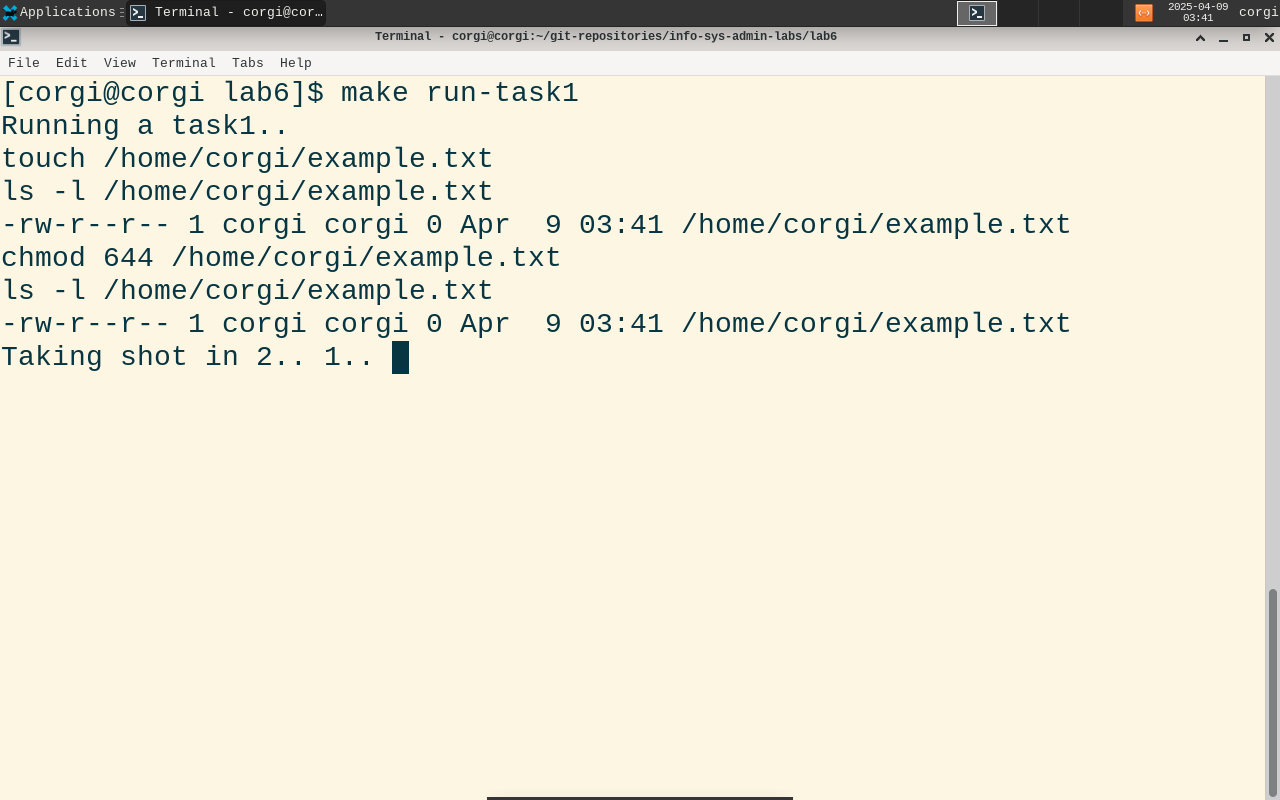
\includegraphics[width=500pt]{task1.png}
		\end{center}
\end{document}
